\paragraph{QuizziPedia::Front-End::ModelViews::QuestionnaireDetailsModelView}
	
	\label{QuizziPedia::Front-End::ModelViews::QuestionnaireDetailsModelView}
	
	\begin{figure}[ht]
		\centering
		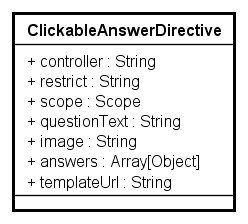
\includegraphics[scale=0.5,keepaspectratio]{UML/Classi/Front-End/QuizziPedia_Front-end_Templates_ClickableAnswerTemplate.png}
		\caption{QuizziPedia::Front-End::ModelViews::QuestionnaireDetailsModelView}
	\end{figure} \FloatBarrier
	
	\begin{itemize}
		\item \textbf{Descrizione}: classe di tipo modelview la cui istanziazione è contenuta all'interno della variabile di ambiente \$scope di \textit{Angular.js\ped{G}}. All'interno di essa sono presenti le variabili e i metodi necessari per il \textit{Two-Way Data-Binding\ped{G}} tra la view \texttt{UserView} e il controller \texttt{QuestionnaireDetailsController};
		\item \textbf{Utilizzo}: viene utilizzata per effettuare il \textit{Two-Way Data-Binding\ped{G}} tra la view \texttt{UserView} e il controller \texttt{QuestionnaireDetailsController} rendendo disponibili variabili e metodi;
		\item \textbf{Relazioni con altre classi}: 
		\begin{itemize}
			\item \textit{IN} \texttt{UserView}: view contenente le direttive dei dati personali dell'utente, delle sue statistiche relative ai questionari e agli allenamenti effettuati e dei questionari a cui è iscritto; 
			\item \textit{IN} \texttt{QuestionnaireDetailsController}: questa classe permette di gestire i dettagli di un questionario;
		\end{itemize}
		\item \textbf{Attributi}: 
		\begin{itemize}
			\item \texttt{+ questionnaireDetails: Object} \\ Oggetto contenente i seguenti campi dati: \texttt{name}, \texttt{author}, \texttt{topic} e \texttt{keywords};\\
			\item \texttt{+ questionnaireDetailsDone: Object} \\ Oggetto contenente i seguenti campi dati: \texttt{name}, \texttt{author}, \texttt{topic}, \texttt{keywords} e \texttt{judgment};
		\end{itemize}
	\end{itemize}
	
		